\paragraph{}{
    Group communication and management is a central part of distributed systems.
This report accounts for the development of \texttt{Gcom}, a middleware that can be used to facilitate group communication as realized in a distributed chat application.
}

\begin{figure}[hb]
	\begin{center}
		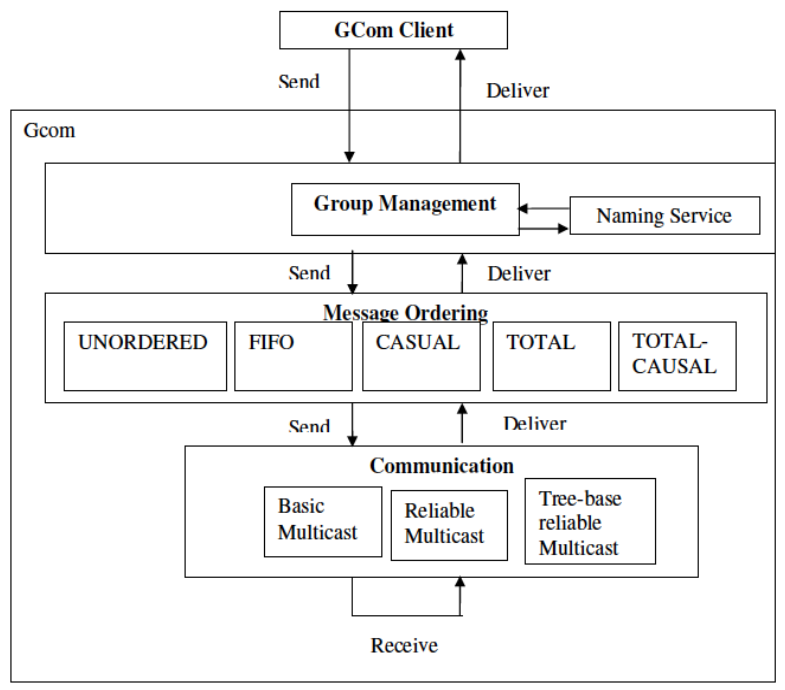
\includegraphics[width=\textwidth]{figures/gcom_intro.png}
	\end{center}
	\caption{
		Overview of the Gcom architecture as given in specification
		\label{fig:gcom_spec}
	}
\end{figure}

\paragraph{}{
Group communication can be broken down to three main modules; Group management, message ordering and communication. These three are layered as shown in Figure \ref{fig:gcom_spec}. For each of these layers there are different algorithms and approaches as to how they function and what behaviour they provide.
Different applications are dependent on different underlying algorithms which means that a group communication middleware should provide easily chosen behaviours in order to be usable.
Gcom is a peer to peer system where all peers have the same responsibility.
}
